%\documentclass[letterpaper,draft]{beamer}
%\documentclass[letterpaper,handout]{beamer}
\documentclass[letterpaper, mathserif]{beamer}

%---multiple pages on one sheet, ADD for handout--
%\usepackage{pgfpages}
%\pgfpagesuselayout{4 on 1}[letterpaper, landscape, border shrink=1mm]
%-------------------------------------------------
\usepackage{amsmath,amsfonts}
\usepackage{colortbl,xcolor}
%\usepackage[misc]{ifsym} % for the dice symbol \Cube{}
%\usepackage{booktabs}
%\usepackage{mdwlist}
%\usepackage{pgf,tikz}
%\usetheme{Copenhagen}
%\usetheme{warsaw}
\setbeamertemplate{navigation symbols}{}
\usepackage[english]{babel}
\def\ul{\underline}
% or whatever

\usepackage[latin1]{inputenc}
\subject{Talks}

\def\Sum{\sum\nolimits}
\def\p{\mathrm P}
\def\E{\mathbb E}
\def\X{\mathfrak{X}}
\def\V{\mathrm{Var}}
%-------------Answers------------
\def\Hide#1#2{\ul{~~~\onslide<#1>{\alert{#2}}~~~}}
\def\hide#1#2{\ul{~~\onslide<#1>{\alert{#2}}~~}}
%------Centered Page Number------
\defbeamertemplate{footline}{centered page number}
{%
  \hspace*{\fill}%
  %\usebeamercolor[fg]{page number in head/foot}%
  %\usebeamerfont{page number in head/foot}%
  \small Lecture \chapnum\ - \insertframenumber%
  \hspace*{\fill}\vskip2pt%
}

%\usepackage{tikz}
%\usebackgroundtemplate{%
%\tikz\node[opacity=0.3] {\includegraphics[height=\paperheight,widht=\paperwidth]{ctanlion}};}

%\usebackgroundtemplate{%
%  %\rule{0pt}{\paperheight}%
%  \parbox[c][\paperheight][c]{\paperwidth}{\centering\includegraphics[width=.65\paperwidth]{UClogo.pdf}}
%  %\hspace*{\paperwidth}
%}

\def\chapnum{6}
%--------------------------------
\setbeamertemplate{footline}[centered page number]

\title{STAT253/317 Lecture \chapnum}
\date{}
\author{Yibi Huang}
\begin{document}
% ----------------------------------------------------------------------
\begin{frame}{STAT253/317 Lecture \chapnum ~ Time Reversibility (\S 4.8)}
\mbox{}
{\bf 4.8.1 Backward Markov Chain}

If $\{\ldots,X_{n-1},X_{n},X_{n+1},\ldots\}$ is a Markov chain,
the \structure{backward} chain $\{\ldots,X_{n+1},X_{n},X_{n-1},\ldots\}$ is also a Markov chain.\smallskip

{\em Proof:}
\begin{align*}
&{}\p(X_m = j~|~{\color{red}X_{m+1} = i},{\color{blue}X_{m+2},X_{m+3}, \ldots})\\[5pt]
=&{}\frac{\p(X_m = j, {\color{red}X_{m+1} = i},{\color{blue}X_{m+2},X_{m+3}, \ldots})}{\p({\color{red}X_{m+1} = i},{\color{blue}X_{m+2},X_{m+3}, \ldots})}\\[5pt]
=&{}\frac{\p({\color{blue}X_{m+2},X_{m+3}, \ldots}~|~X_m = j, {\color{red}X_{m+1} = i})\p(X_m = j, {\color{red}X_{m+1} = i})}{\p({\color{blue}X_{m+2},X_{m+3}, \ldots}~|~{\color{red}X_{m+1} = i})\p({\color{red}X_{m+1} = i})}\\[5pt]
=&{}\frac{\p({\color{blue}X_{m+2},X_{m+3}, \ldots}~|~{\color{red}X_{m+1} = i})\p(X_m = j, {\color{red}X_{m+1} = i})}{\p({\color{blue}X_{m+2},X_{m+3}, \ldots}~|~{\color{red}X_{m+1} = i})\p({\color{red}X_{m+1} = i})}\; (\mbox{Markov Property})\\[5pt]
=&{}\frac{\p(X_m = j, {\color{red}X_{m+1} = i})}{\p({\color{red}X_{m+1} = i})}=\p(X_m = j~|~{\color{red}X_{m+1} = i})
\end{align*}
\end{frame}
% ----------------------------------------------------------------------
\begin{frame}{Transition Probabilities of the Backward Markov Chain}
Consider a Markov chain $\{X_n: n=0,1,2,\ldots\}$ with transition probabilities $\{P_{ij}\}$.

Let $\{\pi^{(m)}_j = P(X_m=j)\}_{j \geq 0}$ be the marginal distribution of $X_m$.

The transition probabilities $\{Q^{(m)}_{ij}\}$ of the backward Markov chain are
\begin{align*}
Q^{(m)}_{ij} &= \p(X_{m}=j~|~X_{m+1}=i)\\
&=\frac{\p(X_{m}=j, X_{m+1}=i)}{\p(X_{m+1}=i)}\\
&=\frac{\p(X_{m}=j)\p(X_{m+1}=i~|~X_{m}=j)}{\p(X_{m+1}=i)}=\frac{\pi^{(m)}_j P_{ji}}{\pi^{(m+1)}_i}
\end{align*}
We can see the backward Markov chain is {\bf NOT stationary} because the transition probabilities $Q^{(m)}_{ij}$ depend on $m$.

\end{frame}
% ----------------------------------------------------------------------
\begin{frame}{How to make a backward Markov chain stationary?}
To make the backward Markov chain {\bf stationary}, the forward chain must start with its stationary distribution
$\{\pi_j\}$ so that
$$
P(X_m=j) = \pi_j \quad\text{for all }m
$$
the transition probabilities $\{Q_{ij}\}$ of the backward Markov chain is
\begin{align*}
Q_{ij} =\frac{\pi_j P_{ji}}{\pi_i}
\end{align*}
which does not depend on $m$
\end{frame}
% ----------------------------------------------------------------------
\begin{frame}{Time Reversible Markov Chains \& Detailed Balanced Equations}
A Markov chain is said to be \structure{\em time reversible} iff $$Q_{ij}=P_{ij},$$
i.e., {\bf it behaves exactly the same} no matter {\bf running forward or backward} when in the stationary state.\par\medskip

Because $Q_{ij}$ equals $\pi_j P_{ji}/\pi_i$, a Markov chain is time reversible if and only if
its stationary distribution $\{\pi_j\}$ satisfies the equations
$$\pi_i P_{ij}=\pi_j P_{ji}\quad\mbox{for all}\ i,j.$$
This set of equations is called the {\bf detailed balanced equation}.
\end{frame}
% ----------------------------------------------------------------------
\begin{frame}{Balanced Equations v.s. Detailed Balanced Equations}
Recall a distribution ${\pi_j}$ for a Markov chain is said to be stationary if and only if
it satisfies
$$\pi_j = \sum_{i\in\X}\pi_i P_{ij}\quad\text{for all }j\in\X.$$
This set of equations is called the {\bf balanced equations}.\pause

\medskip\hrule\medskip
A solution to the {\bf detailed balanced equations}
must also be a solution to the {\bf balanced equations}, because
$$
\Sum_{i\in\mathfrak{X}}\pi_i P_{ij}=\Sum_{i\in\mathfrak{X}}\pi_j P_{ji}
=\pi_j\Sum_{i\in\mathfrak{X}}P_{ji}=\pi_j\cdot 1=\pi_j
$$\pause
\medskip\hrule\medskip
It is possible that the balanced equations have solutions but
the detailed balanced equations do not.
\end{frame}
% ----------------------------------------------------------------------
\begin{frame}{Interpretation of the Balanced Equation}
\begin{align*}
\pi_j &= \sum_{i\in\X}\pi_i P_{ij}\quad\text{for all }j\in\X\\
\Leftrightarrow\quad\pi_j(1-P_{jj}) &= \sum_{i\in\X, i\neq j}\pi_i P_{ij}\quad\text{for all }j\in\X
\end{align*}
\begin{center}
\fbox{rate of transitions \textbf{out of} state $j=$ rate of transitions \textbf{into} state $j$}
\end{center}
$$
\arraycolsep=3pt
\begin{array}{c@{\,}rcl@{\,}c}
~~~\bullet& & \bullet &  &\bullet~~~\\
&\nwarrow&\uparrow&\nearrow&\\
\bullet~~~&\longleftarrow & j & \longrightarrow &~~\bullet\\
&\swarrow&\downarrow&\searrow&\\
~~~\bullet& &\bullet &  &\bullet~~~\\
\end{array}
\qquad\qquad
\begin{array}{c@{\,}rcl@{\,}c}
~~~\bullet& & \bullet &  &\bullet~~~\\
&\searrow&\downarrow&\swarrow&\\
\bullet~~~&\longrightarrow & j & \longleftarrow & ~~\bullet\\
&\nearrow&\uparrow&\nwarrow&\\
~~~\bullet& &\bullet &  &\bullet~~~
\end{array}
$$

\end{frame}
% ----------------------------------------------------------------------
\begin{frame}{Interpretation of the Detailed Balanced Equation}
$$\pi_i P_{ij}=\pi_j P_{ji}$$
\begin{center}
\fbox{rate of transitions from $i$ to $j=$ rate of transitions from $j$ to $i$}
\end{center}
$$
i\longrightarrow j\qquad\qquad j\longrightarrow i
$$
\end{frame}
% ----------------------------------------------------------------------
\begin{frame}{Balanced Eqns v.s. Detailed Balanced Eqns.}

\begin{itemize}
\item For balanced equations, 
\begin{center}the \# of equations = \# of states = \# of unknowns\end{center}
\item For detailed balanced equations,
\begin{center}\# of equations = \# of pairs of states $>$ \# of unknowns\end{center}
\item Detailed Balanced Equations are easier to solve than the Balanced Equations 
as the former ones involve only two unknowns in each equation
\item One can start by solving the detailed balanced equations for the stationary distribution.
If you can find one, it'll also be the solution for the balanced equations.
That also proves the Markov chain if positive recurrent if it's irreducible (2nd limit theorem).
\item However, if the detailed balanced equations have no solutions, 
it doesn't prove the Markov chain to be null current or transient since
the balanced equations might still have a solution.
\end{itemize}
\end{frame}
% ----------------------------------------------------------------------
\begin{frame}{Example 4.35}
Consider a random walk with states $0, 1,\ldots,M$ and transition
probabilities
\begin{align*}
P_{i,i+1} &= \alpha_i = 1 -P_{i,i-1},\quad\text{for } i= 1, \ldots , M - 1,\\
P_{0,1}   &= \alpha_0 = 1 -P_{0,0},\\
P_{M,M}   &= \alpha_M = 1 -P_{M,M-1}
\end{align*}
$$
\begin{array}{cc}
0 \stackrel{\alpha_0}{\longrightarrow}
1 \stackrel{\alpha_1}{\longrightarrow}
2\cdots \longrightarrow
M-1\stackrel{\alpha_{M-1}}{\longrightarrow}&M\\[-3pt]
& {\text{\Large$\circlearrowleft$}}\\[-6pt]
&{\text{\scriptsize$\alpha_M$}}
\end{array}
$$

$$
\begin{array}{c@{\hspace{0pt}}c}
0 &\stackrel{1-\alpha_1}{\longleftarrow}
1 \stackrel{1-\alpha_2}{\longleftarrow}
2\cdots \longleftarrow
M-1\stackrel{1-\alpha_{M}}{\longleftarrow}M\\[-3pt]
{\text{\Large$\circlearrowleft$}}&\\[-6pt]
{\text{\scriptsize$1-\alpha_0$}}&
\end{array}
$$

\end{frame}
% ----------------------------------------------------------------------
\begin{frame}{Example 4.35 (Cont'd)}
The stationary distribution $\pi$ can be solved via the detailed balanced equation
$$\pi_iP_{i,i-1}=\pi_i(1-\alpha_{i}) =\pi_{i-1}P_{i-1,i}=\pi_{i-1}\alpha_{i-1}$$
So
$$
\pi_{i}=\frac{\alpha_{i-1}}{1-\alpha_{i}}\pi_{i-1}=\ldots
=\frac{\alpha_{i-1}\alpha_{i-2}\ldots\alpha_{0}}{(1-\alpha_{i})(1-\alpha_{i-1})\ldots(1-\alpha_1)}\pi_0
$$
Since $\sum_0^M \pi_i=1$, one can solve $\pi_0$ via
$$
\pi_0\left[1+\Sum_{i=1}^M\frac{\alpha_{i-1}\alpha_{i-2}\ldots\alpha_{0}}{(1-\alpha_{i})(1-\alpha_{i-1})\ldots(1-\alpha_1)}\right]=1
$$
\end{frame}
% ----------------------------------------------------------------------
\begin{frame}{A Non-Time-Reversible Markov Chain}
In Exercise 4.34 (a flea moving around the vertices of a triangle), 
$$
\arraycolsep=2pt
\begin{array}{ccccc}
&&1&&\\
&\stackrel{p_3}{\nearrow}&&\stackrel{p_1}{\searrow}\\
3&&\stackrel{p_2}{\longleftarrow}&& 2
\end{array}\quad\quad
\begin{array}{ccccc}
&&1&&\\
&\stackrel{q_1}{\swarrow}&&\stackrel{q_2}{\nwarrow}\\
3&&\stackrel{q_3}{\longrightarrow}&& 2
\end{array}\quad\text{where }p_i+q_i=1
$$
the transition probabilities,
and the stationary distribution are respectively
$$
\bordermatrix{%
 & 1  & 2   & 3\cr
1& 0  & p_1 & q_1\cr
2&q_2 & 0   & p_2\cr
3&p_3 & q_3 & 0
},
\quad\mbox{and}\; \pi=(\frac{1-p_2q_3}{C},\frac{1-p_3q_1}{C},\frac{1-p_1q_2}{C})
$$
where $C=3-p_2q_3-p_3q_1-p_1q_2$. One can easily verify that
$$
\pi_1 P_{12}=\pi_1 p_1\neq \pi_2 P_{21}=\pi_2 q_2
$$
\begin{center}
The chain is NOT time reversible.
\end{center}
\end{frame}
% ----------------------------------------------------------------------
\begin{frame}{Other Non-Time-Reversible Markov Chains}
\begin{itemize}
\item A Markov chain with {\bf transient states} cannot be time-reversible because then running forward and backward in time will not be equivalent.\vspace{40pt}
\item If there exists two states $i$ and $j$ such that
$$P_{ij}>0\quad\text{but}\quad P_{ji}=0$$
then the Markov chain cannot be time-reversible because then when running backward in time
$$Q_{ij}=\frac{\pi_j P_{ji}}{\pi_i}=0\neq P_{ij}.$$
\end{itemize}
\end{frame}
% ----------------------------------------------------------------------
\begin{frame}{Theorem 4.2}
An ergodic Markov chain for which $P_{ij} = 0$ whenever $P_{ji} = 0$ is
time reversible if and only if starting in state $i$, any path back to $i$ has the same
probability as the reversed path. That is, if
$$P_{ii_1}P_{i_1i_2}\ldots P_{i_ki} = P_{ii_k}P_{i_ki_{k-1}}\ldots P_{i_1i} $$
for all states $i, i_1,\ldots, i_k$.
$$
\arraycolsep=2pt
\begin{array}{rcccccc}
&& i_k & \longrightarrow & i & \\
&\nearrow&&&&\searrow&\\
i_{k-1} &&&&&& i_1\\
&\nwarrow&&&&\swarrow&\\
&& \cdots & \longleftarrow & i_2 & 
\end{array}
\qquad\quad
\begin{array}{ccccccc}
&& i_k & \longleftarrow & i & \\
&\swarrow&&&&\nwarrow&\\
i_{k-1} &&&&&& i_1\\
&\searrow&&&&\nearrow&\\
&& \cdots & \longrightarrow & i_2 & 
\end{array}
$$
\end{frame}
% ----------------------------------------------------------------------
\begin{frame}{Theorem 4.2 --- Proof of Necessity}

If a Markov chain is time reversible, we have
$$\pi_iP_{ij} = \pi_jP_{ji},\quad \pi_kP_{kj} = \pi_jP_{jk}.$$
implying (if $P_{ij}P_{jk} > 0$) that
$$\frac{\pi_i}{\pi_k}= \frac{P_{ji}P_{kj}}{P_{ij}P_{jk}},$$
but $\pi_iP_{ik} = \pi_kP_{ki}$ also implies $\pi_i/\pi_k=P_{ki}/P_{ik}$.
Thus $$P_{ik}P_{kj}P_{ji} = P_{ij}P_{jk}P_{ki}.$$
This proves for the case $i\to j\to k\to i$.
The general case for longer cycle can be proved similarly
\end{frame}
% ----------------------------------------------------------------------
\begin{frame}{Theorem 4.2 --- Proof of Sufficiency}

Consider the cycle $i\to i_1\to i_2\to\ldots\to i_k\to j\to i$.
$$P_{ii_1}P_{i_1i_2}\ldots P_{i_kj}P_{ji} = P_{ij}P_{ji_k}P_{i_ki_{k-1}}\ldots P_{i_1i}$$
Summing the preceding over all states $i_1,\ldots, i_k$ yields
$$P^{(k)}_{ij} P_{ji} = P_{ij}P^{(k)}_{ji}$$
Letting $k\to\infty$ yields
$$\underbrace{\lim_{k\to\infty} P^{(k)}_{ij}}_{=\pi_j} P_{ji} = P_{ij}\underbrace{\lim_{k\to\infty} P^{(k)}_{ji}}_{=\pi_i}$$
in which $\lim_{k\to\infty} P^{(k)}_{ij}=\pi_j$ for all $j$ since the Markov chain is ergodic.

This proves the theorem.
\end{frame}
% ----------------------------------------------------------------------
\begin{frame}{Example 4.36 Random Walk on a Weighted Graph (p.241)}
\begin{center}
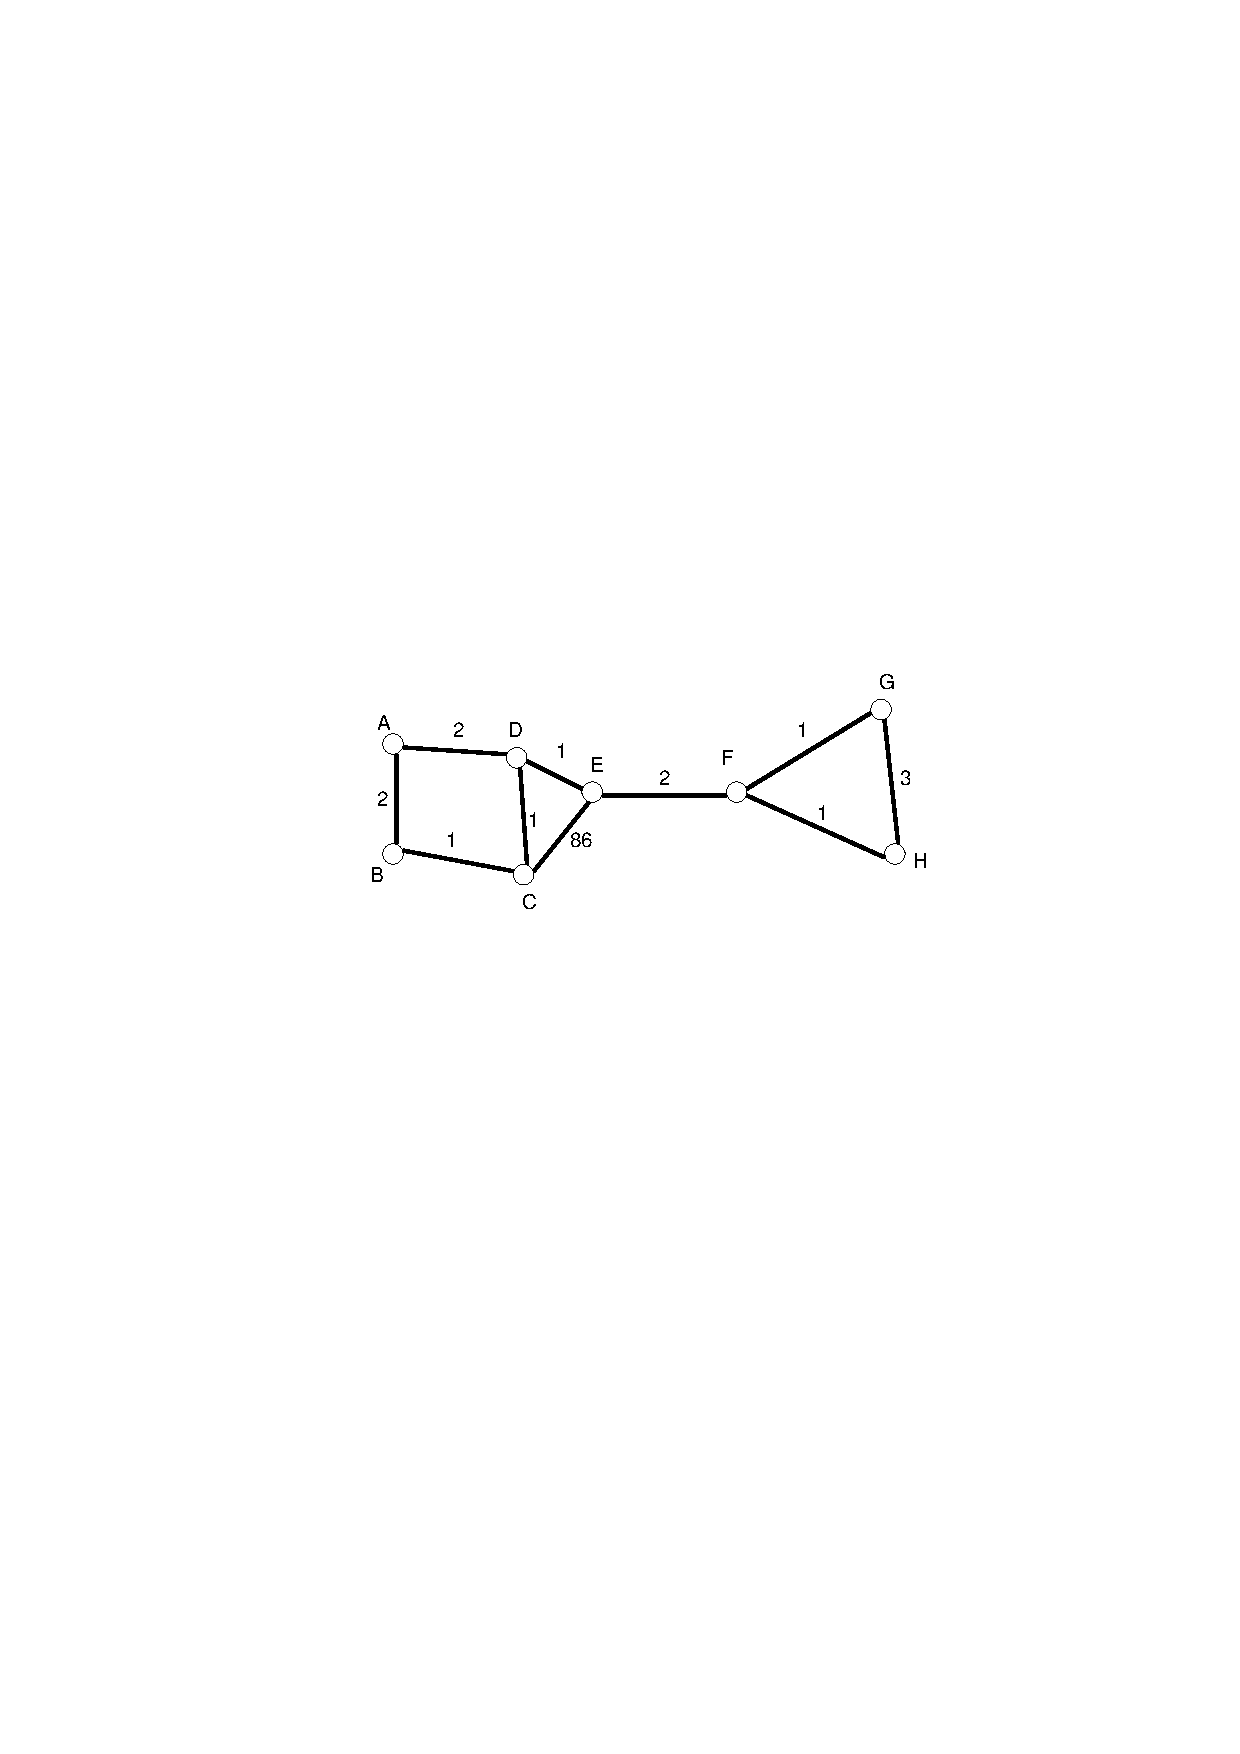
\includegraphics[width=0.6\textwidth]{WeightedGraph}
\end{center}
A graph = a set of \structure{vertices} (or \structure{nodes}) + a set of  \structure{arcs} (or \structure{edges}) connecting some pairs of vertices. We consider random walk on a connected graph such that
\begin{itemize}
\item each pair $(i,j)$ of vertices are connected by at most one arc;
\item all arcs are \structure{undirected}: arc $(i,j)$ = arc $(j,i)$;
\item there is a path consists of arcs connecting any pair of vertices;
\item each arc $(i,j)$ is associated with a \structure{weight} $w_{ij}>0$
\begin{itemize}
\item $w_{ij}=0$ if there is not arc connecting $(i,j)$
\item $w_{ij}=w_{ji}$
\end{itemize}
\end{itemize}
\end{frame}
% ----------------------------------------------------------------------
\begin{frame}{Example 4.36 Random Walk on a Weighted Graph (p.241)}
A particle moving from vertices to vertices that
if at any time the particle is at node $i$, then it will next move to node $j$
with probability
\[
P_{ij} = \frac{w_{ij}}{\sum_k w_{ik}},
\]
E.g., in the graph below, there are two arcs from vertices $B$ with weights $w_{BA}=2$  and $W_{BC}=1$ respectively.
So,
{\small
\[P_{BA}=\frac{w_{BA}}{w_{BA}+w_{BC}}=\frac{2}{2+1}=\frac{2}{3},\quad P_{BC}=\frac{w_{BC}}{w_{BA}+w_{BC}}=\frac{1}{2+1}=\frac{1}{3}.\]}
\begin{center}
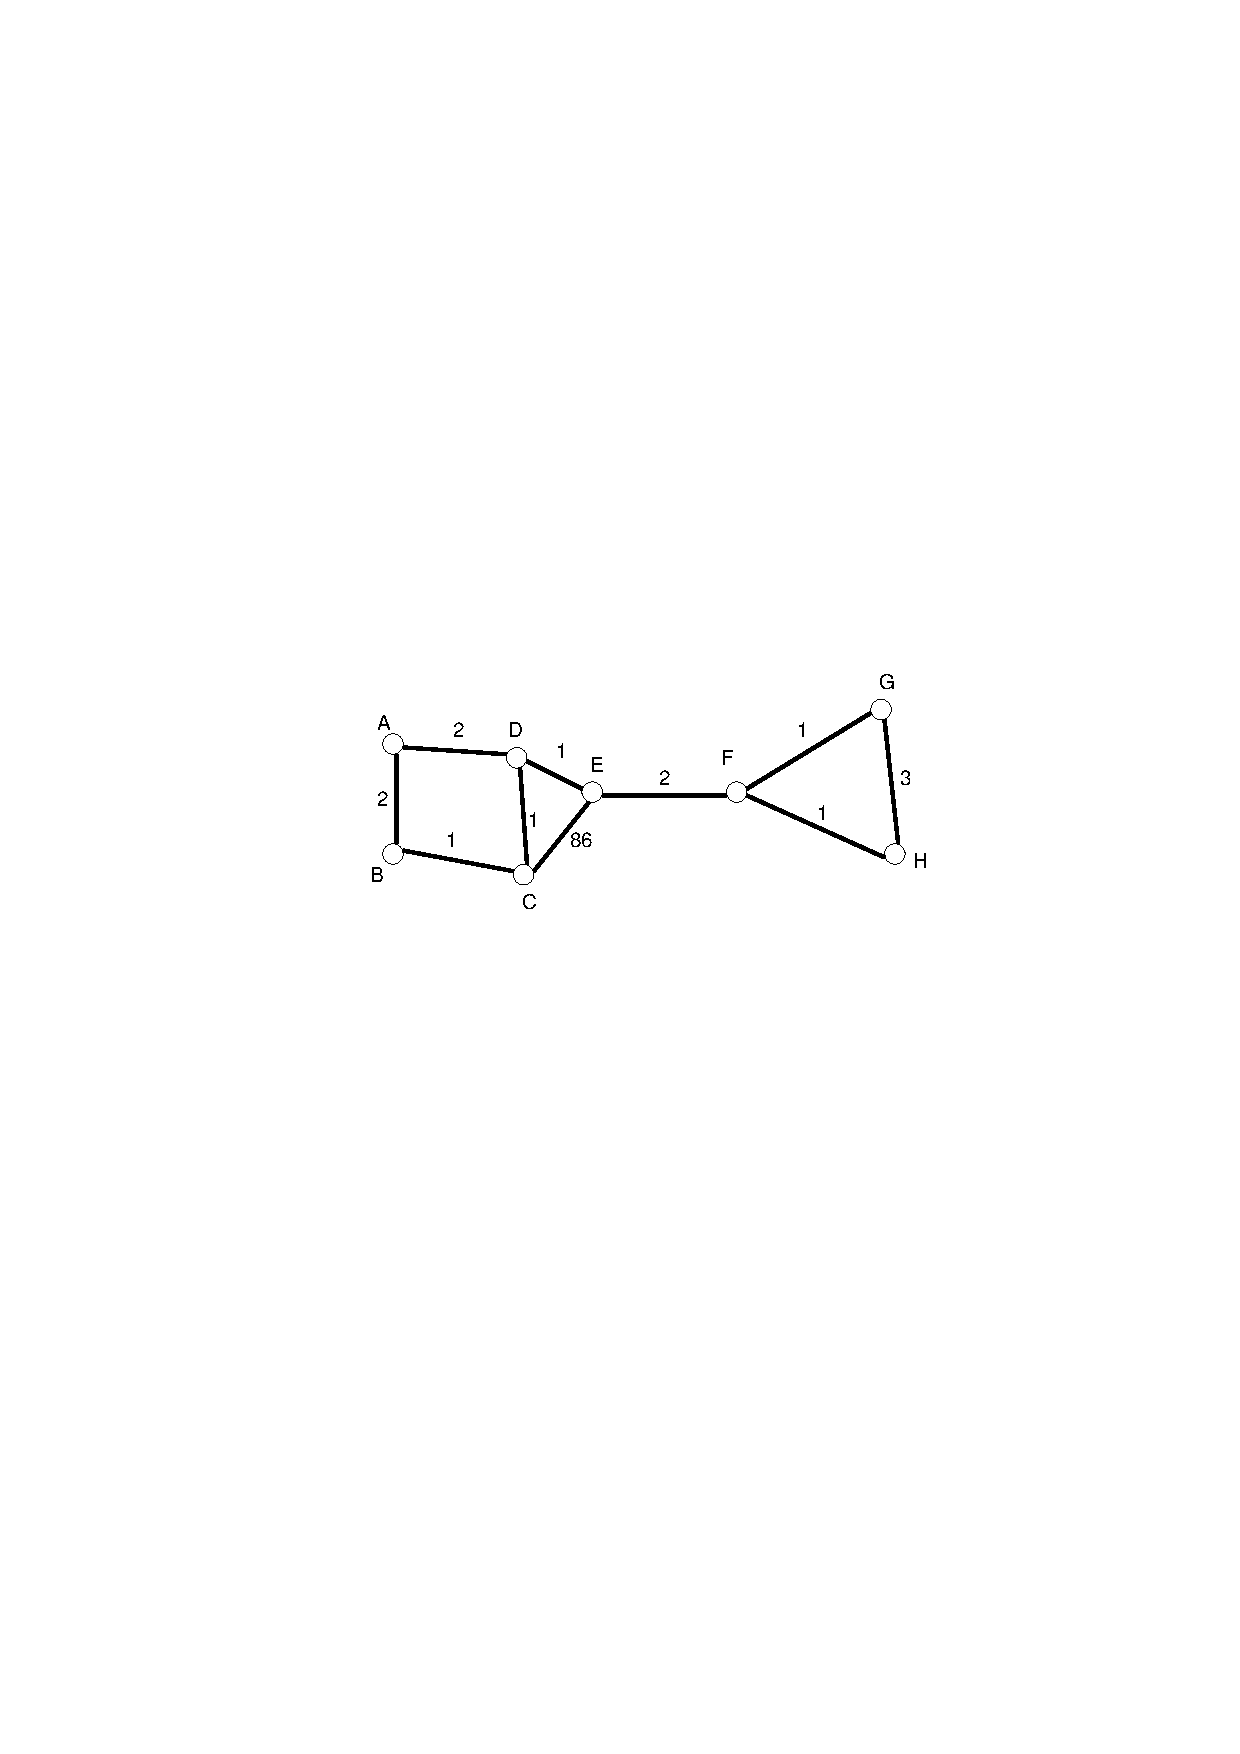
\includegraphics[width=0.65\textwidth]{WeightedGraph}
\end{center}
Random walk on a graph is {\bf irreducible} because the graph is {\bf connected}.
\end{frame}
% ----------------------------------------------------------------------
\begin{frame}{Random Walk on a Weighted Graph is Time Reversible}
Solving the detailed balanced equation:
\[
\pi_iP_{ij}=\frac{\pi_iw_{ij}}{\sum_k w_{ik}}=\frac{\pi_jw_{ji}}{\sum_k w_{jk}}=\pi_jP_{ji}\quad\text{for all }i, j
\]
or, equivalently, since $w_{ij}=w_{ji}$,
\[
\frac{\pi_i}{\sum_k w_{ik}}=\frac{\pi_j}{\sum_k w_{jk}}\quad\text{for all }i, j,
\]
which means $\dfrac{\pi_i}{\sum_k w_{ik}}$ is a constant $c$ for all $i$, i.e.,
\[
\pi_i=c\sum_k w_{ik}.
\]
Since $1=\sum_j\pi_j=c\sum_j\sum_k w_{jk},$ we know $c = 1/(\sum_j\sum_k w_{jk})$, and hence
\[
\pi_i=\frac{\sum_k w_{ik}}{\sum_j\sum_k w_{jk}}
\]
is a solution to the detailed balanced eq. The process is therefore \structure{time-reversible}.
\end{frame}
% ----------------------------------------------------------------------
\begin{frame}{Random Walk on a Weighted Graph}
\begin{center}
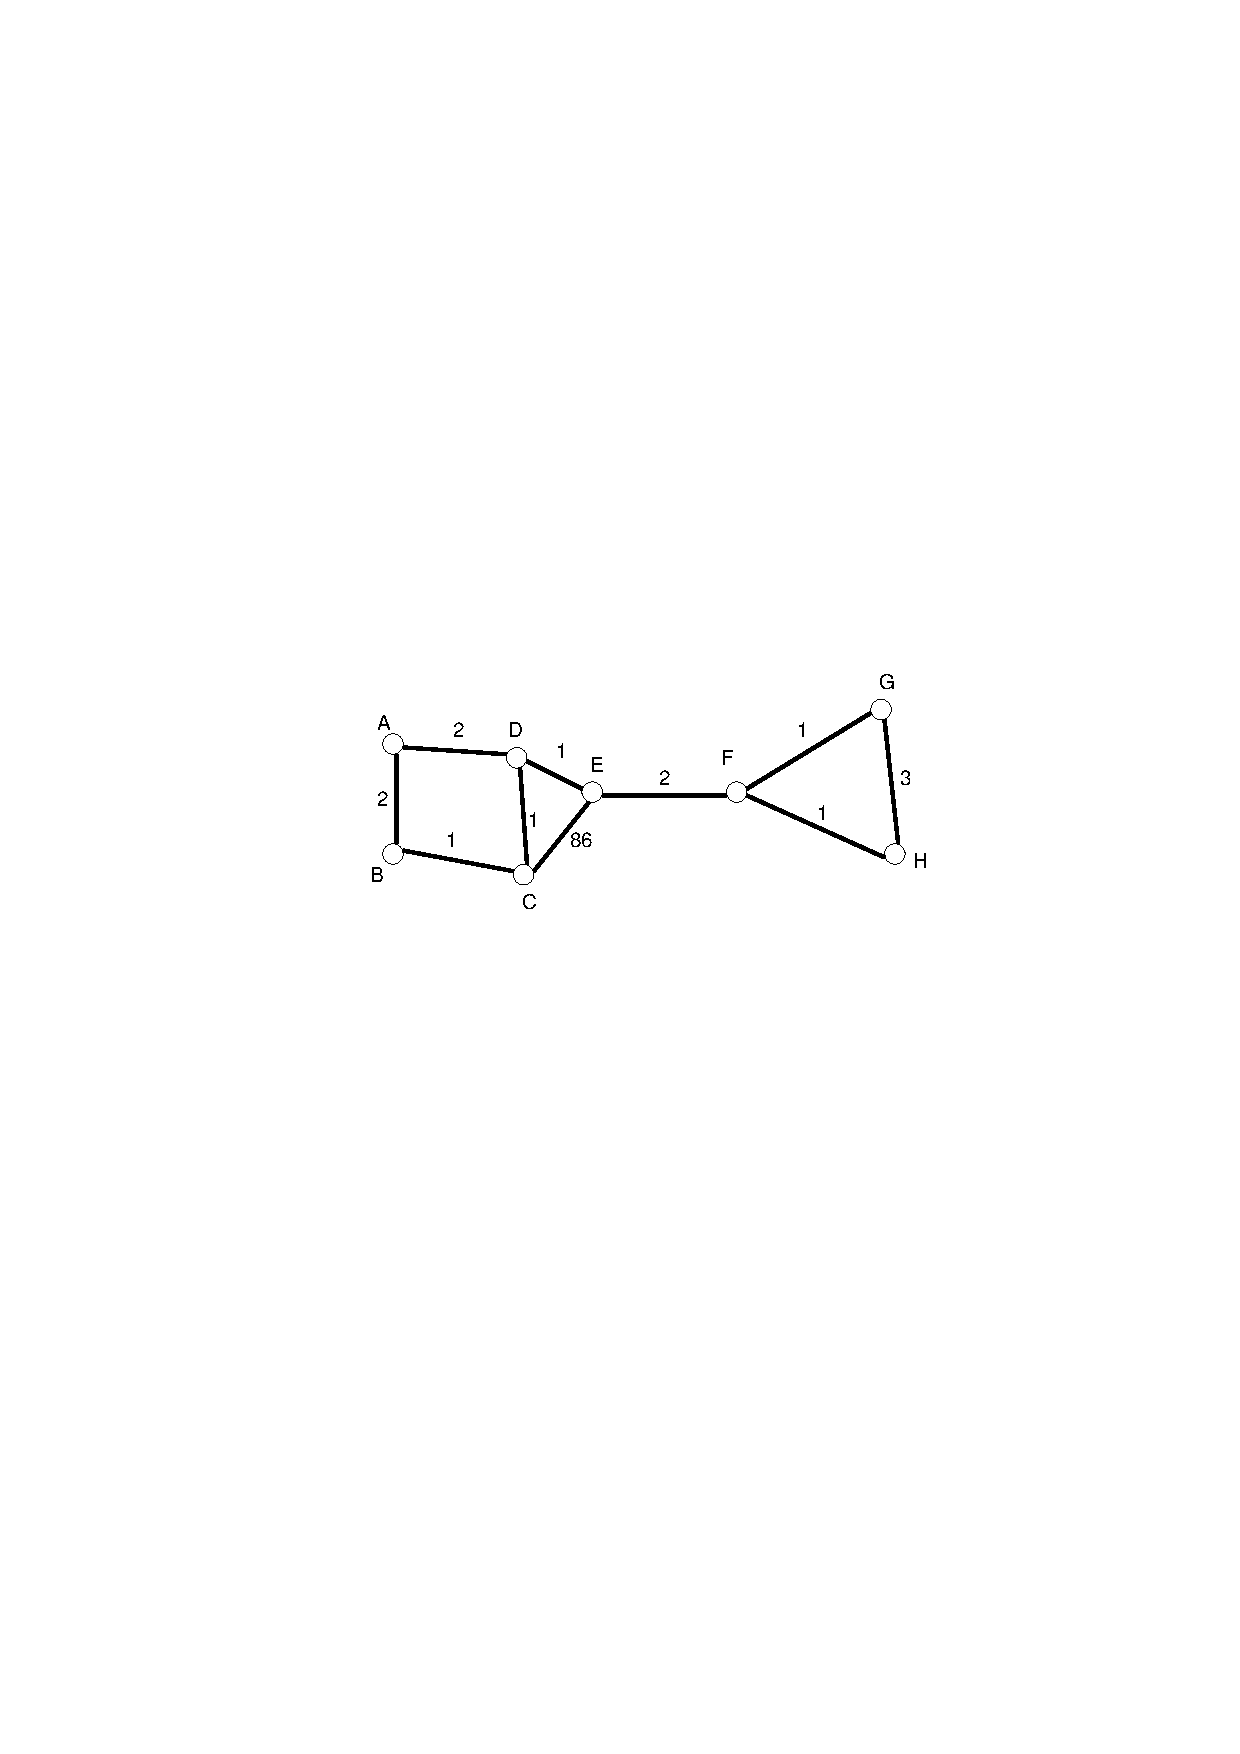
\includegraphics[width=0.6\textwidth]{WeightedGraph}

\small
\begin{tabular}{crc}
Vertices $i$ & $\sum_k w_{ik}$ & $\pi_i$\\\hline
A & $2+2=4$     & $\pi_A=4/200$\\\
B & $2+1=3$     & $\pi_B=3/200$\\
C & $1+1+86=88$ & $\pi_C=88/200$\\
D & $2+1+1=4$   & $\pi_D=4/200$\\
E & $1+2+86=89$ & $\pi_E=89/200$\\
F & $2+1+1=4$   & $\pi_F=4/200$\\
G & $1+3=4$     & $\pi_G=4/200$\\
H & $1+3=4$     & $\pi_H=4/200$\\\hline
Sum &$\sum_i\sum_k w_{ik}=200$ &
\end{tabular}
\end{center}
\end{frame}
% ----------------------------------------------------------------------
\begin{frame}{Random Knight on a Chessboard}

\begin{columns}
\begin{column}{0.28\textwidth}
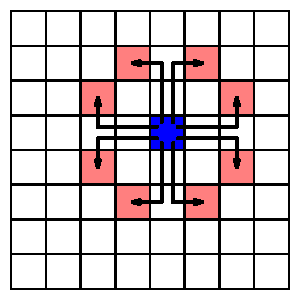
\includegraphics[width=1.2\textwidth]{./RandomKnight/KnightMoves44}
\end{column}
\begin{column}{0.7\textwidth}
\hspace{-20pt}\begin{itemize}
\item The Knight moves in an \alert{\bf L} shape in any direction.
\item At the {\color{blue} blue square}, the Knight
can move to any of the 8 {\color{red} red squares}.
\item From a square near the boundary, the Knight has fewer possible
moves as it cannot move out of the Chessboard (see the 3 graphs below.)
\end{itemize}
\end{column}
\end{columns}
\medskip

\tabcolsep=0pt
\begin{tabular}{ccc}
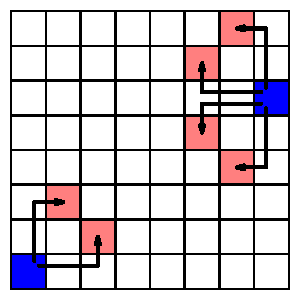
\includegraphics[width=0.33\textwidth]{./RandomKnight/KnightMoves_Border}
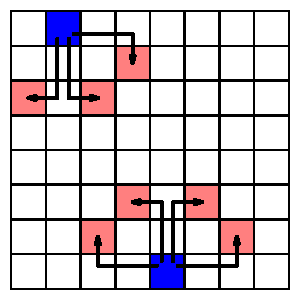
\includegraphics[width=0.33\textwidth]{./RandomKnight/KnightMoves_Border2}
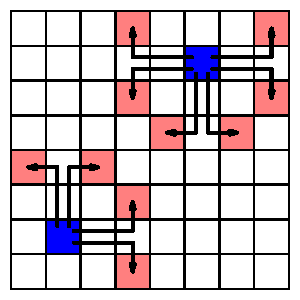
\includegraphics[width=0.33\textwidth]{./RandomKnight/KnightMoves_Border3}
\end{tabular}
\end{frame}
% ----------------------------------------------------------------------
\begin{frame}{Random Knight on a Chessboard}
\begin{itemize}
\item A Knight moves randomly on an empty chessboard.
\item In each step, it's equally like to take any of its legal moves. E.g.,
at the corner, it has prob. 1/2 each to move to either of the two red squares,
from which it has prob. 1/6 each to move to any of the 6 possible squares.
\begin{center}
\begin{tabular}{cc}
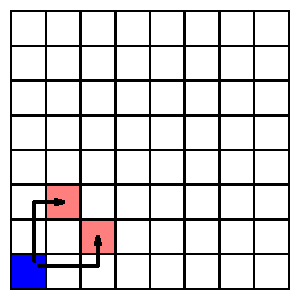
\includegraphics[width=0.33\textwidth]{./RandomKnight/KnightMoves00}
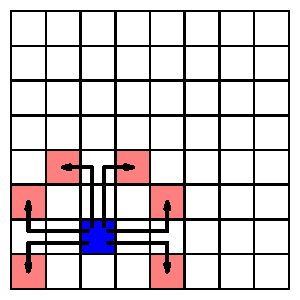
\includegraphics[width=0.33\textwidth]{./RandomKnight/KnightMoves21}
\end{tabular}
\end{center}
\item Each move is indep. of the history of moves up to that time.
\item The position of on knight after $n$th move
is a Markov chain where states are the 64 squares on the chessboard.
\end{itemize}
\end{frame}
% ----------------------------------------------------------------------
\begin{frame}{Random Knight on a Chessboard}
The Knight's random walk on a Chessboard is also a random walk on weighted graph where
\begin{itemize}
\item the vertices are the 64 squares on the chessboard;
\item there is an arc between any two squares that Knight can move in 1 step;
\item all the arcs have weight $w_{ij}=1$.
\end{itemize}
The transition probability of a random walk on weighted graph from square $i$ to square $j$ is
\begin{align*}
P_{ij} = \frac{w_{ij}}{\sum_k w_{ik}}
&= \frac{1}{\text{\# of squares that connected with square $i$ with an arc}}\\
&= \frac{1}{\text{\# of legal moves from square $i$}}
\end{align*}
which is exactly the random walk of the knight.
\end{frame}
% ----------------------------------------------------------------------
\begin{frame}{Random Knight on a Chessboard}
Using the property of random walks on a graph, the stationary distribution of the Knight's random walk is
\[
\pi_i=\frac{\sum_k w_{ik}}{\sum_j\sum_k w_{jk}}=\frac{{\text{\# of legal moves from square $i$}}}{\sum_j (\text{\# of legal moves from square $j$})}
\]

The numbers of legal moves from the squares are as follows:\smallskip

\begin{columns}
\begin{column}{0.4\textwidth}
\small\tabcolsep=5pt
\begin{tabular}{|c|c|c|c|c|c|c|c|}\hline
\cellcolor{orange}2 & \cellcolor{yellow}3 & \cellcolor{pink}4 & \cellcolor{pink}4 & \cellcolor{pink}4 & \cellcolor{pink}4 & \cellcolor{yellow}3 & \cellcolor{orange}2\\\hline
\cellcolor{yellow}3 & \cellcolor{pink}4 & \cellcolor{cyan}6 & \cellcolor{cyan}6 & \cellcolor{cyan}6 & \cellcolor{cyan}6 & \cellcolor{pink}4 & \cellcolor{yellow}3\\\hline
\cellcolor{pink}4 & \cellcolor{cyan}6 & 8 & 8 & 8 & 8 & \cellcolor{cyan}6 & \cellcolor{pink}4\\\hline
\cellcolor{pink}4 & \cellcolor{cyan}6 & 8 & 8 & 8 & 8 & \cellcolor{cyan}6 & \cellcolor{pink}4\\\hline
\cellcolor{pink}4 & \cellcolor{cyan}6 & 8 & 8 & 8 & 8 & \cellcolor{cyan}6 & \cellcolor{pink}4\\\hline
\cellcolor{pink}4 & \cellcolor{cyan}6 & 8 & 8 & 8 & 8 & \cellcolor{cyan}6 & \cellcolor{pink}4\\\hline
\cellcolor{yellow}3 & \cellcolor{pink}4 & \cellcolor{cyan}6 & \cellcolor{cyan}6 & \cellcolor{cyan}6 & \cellcolor{cyan}6 & \cellcolor{pink}4 & \cellcolor{yellow}3\\\hline
\cellcolor{orange}2 & \cellcolor{yellow}3 & \cellcolor{pink}4 & \cellcolor{pink}4 & \cellcolor{pink}4 & \cellcolor{pink}4 & \cellcolor{yellow}3 & \cellcolor{orange}2\\\hline
\end{tabular}
\end{column}
\begin{column}{0.58\textwidth}
The sum of the number of possible moves over all squares is
\begin{align*}
&2\times4+3\times8+4\times20\\
&\quad+6\times16+8\times 16=336.
\end{align*}
\end{column}
\end{columns}
\medskip

The long run proportion of time that the Knight is in a specific square is
simply the counts in the table above divided by 336.

\end{frame}
% ----------------------------------------------------------------------
\begin{frame}{Return Time of a Random Knight}
Recall that $1/\pi_i=\E[T_i]$ is the expected time between two visits of the Markov chain to state $i$.

\begin{minipage}{0.7\linewidth}Starting from one of the four corners,
 it takes $1/\pi_i=336/2=168$ moves on average for a Knight to return to its initial position.
 \end{minipage}
\begin{minipage}{0.28\linewidth}\tabcolsep=3pt
\begin{flushright}
\renewcommand{\arraystretch}{0.65}
\begin{tabular}{|c|c|c|c|c|c|c|c|}\hline
\cellcolor{orange}~ & ~ & ~ & ~ & ~ & ~ & ~ & \cellcolor{orange}~ \\\hline
~ & ~ & ~ & ~ & ~ & ~ & ~ & ~ \\\hline
~ & ~ & ~ & ~ & ~ & ~ & ~ & ~ \\\hline
~ & ~ & ~ & ~ & ~ & ~ & ~ & ~ \\\hline
~ & ~ & ~ & ~ & ~ & ~ & ~ & ~ \\\hline
~ & ~ & ~ & ~ & ~ & ~ & ~ & ~ \\\hline
~ & ~ & ~ & ~ & ~ & ~ & ~ & ~ \\\hline
\cellcolor{orange}~ & ~ & ~ & ~ & ~ & ~ & ~ & \cellcolor{orange}~\\\hline
\end{tabular}
\end{flushright}
\end{minipage}\bigskip  

\begin{minipage}{0.7\linewidth}Starting from the center of the chessboard,
 it takes $1/\pi_i=336/8=42$ moves on average for a Knight to return to its initial position
 \end{minipage}
\begin{minipage}{0.28\linewidth}\tabcolsep=3pt
\begin{flushright}
\renewcommand{\arraystretch}{0.65}
\begin{tabular}{|c|c|c|c|c|c|c|c|}\hline
~ & ~ & ~ & ~ & ~ & ~ & ~ & ~ \\\hline
~ & ~ & ~ & ~ & ~ & ~ & ~ & ~ \\\hline
~ & ~ & \cellcolor{yellow}~ & \cellcolor{yellow}~ & \cellcolor{yellow}~ & \cellcolor{yellow}~ & ~ & ~ \\\hline
~ & ~ & \cellcolor{yellow}~ & \cellcolor{yellow}~ & \cellcolor{yellow}~ & \cellcolor{yellow}~ & ~ & ~ \\\hline
~ & ~ & \cellcolor{yellow}~ & \cellcolor{yellow}~ & \cellcolor{yellow}~ & \cellcolor{yellow}~ & ~ & ~ \\\hline
~ & ~ & \cellcolor{yellow}~ & \cellcolor{yellow}~ & \cellcolor{yellow}~ & \cellcolor{yellow}~ & ~ & ~ \\\hline
~ & ~ & ~ & ~ & ~ & ~ & ~ & ~ \\\hline
~ & ~ & ~ & ~ & ~ & ~ & ~ & ~\\\hline
\end{tabular}
\end{flushright}
\end{minipage}
\end{frame}
% ----------------------------------------------------------------------
\begin{frame}{More Questions}
\begin{itemize}
\item Is this Markov chain irreducible? That is, can the Knight visit every square from every square?\bigskip
\item What is the period of this Markov chain?\pause

\begin{flushleft}
\begin{tabular}{|c|c|c|c|c|c|c|c|}\hline
\cellcolor{gray}~ & ~ & \cellcolor{gray}~ & ~ & \cellcolor{gray}~ & ~ & \cellcolor{gray}~ & ~ \\\hline
~ & \cellcolor{gray}~ & ~ & \cellcolor{gray}~ & ~ & \cellcolor{gray}~ & ~ & \cellcolor{gray}~ \\\hline
\cellcolor{gray}~ & ~ & \cellcolor{gray}~ & ~ & \cellcolor{gray}~ & ~ & \cellcolor{gray}~ & ~ \\\hline
~ & \cellcolor{gray}~ & ~ & \cellcolor{gray}~ & ~ & \cellcolor{gray}~ & ~ & \cellcolor{gray}~ \\\hline
\cellcolor{gray}~ & ~ & \cellcolor{gray}~ & ~ & \cellcolor{gray}~ & ~ & \cellcolor{gray}~ & ~ \\\hline
~ & \cellcolor{gray}~ & ~ & \cellcolor{gray}~ & ~ & \cellcolor{gray}~ & ~ & \cellcolor{gray}~ \\\hline
\cellcolor{gray}~ & ~ & \cellcolor{gray}~ & ~ & \cellcolor{gray}~ & ~ & \cellcolor{gray}~ & ~ \\\hline
~ & \cellcolor{gray}~ & ~ & \cellcolor{gray}~ & ~ & \cellcolor{gray}~ & ~ & \cellcolor{gray}~\\\hline
\end{tabular}
\end{flushleft}
\pause


\textcolor{red}{Every ``L'' move can only from a gray square to a white square or a white square to a gray square.}

\end{itemize}
\end{frame}
% ----------------------------------------------------------------------
\end{document}